%% =========================================================================
%% Master's Dissertation — PPGCC, CIn-UFPE — ENGLISH VERSION
%% Template: risethesis (CIn class), option [en]
%% Adapted (not literally translated) from dissertacao/, which remains the
%% deposit reference; this version targets international dissemination.
%% Compile: tectonic main.tex (or pdflatex -> bibtex -> pdflatex x2)
%% =========================================================================
\documentclass[en,oneside,onehalfspacing,msc]{risethesis}

\usepackage{babel}% the class passes [brazil,english]; english is primary
\usepackage{color}
\usepackage[table]{xcolor}
\usepackage{microtype}
\usepackage{multirow}
\usepackage{rotating}
\usepackage{booktabs}
\usepackage{caption}
\usepackage{float}
\usepackage{subcaption}
\usepackage{amsmath,amssymb}
\usepackage{textcomp}
% Escape valve for paragraphs with long tokens (artifact paths in \texttt):
\emergencystretch=1.5em
% tikz is not in the preamble: diagrams are pre-compiled into
% images/tikz-*-en.pdf (editable sources in tikz-src/).
\setcounter{secnumdepth}{3}
\setcounter{tocdepth}{2}

%% ---- Title format following the CIn dissertation standard ----
\titleformat{\chapter}[hang]
  {\normalsize\bfseries}{\thechapter}{1em}{\MakeUppercase}
\titleformat{name=\chapter,numberless}[hang]
  {\normalsize\bfseries\filcenter}{}{0pt}{\MakeUppercase}
\titlespacing*{\chapter}{0pt}{0pt}{24pt}
\titleformat{\section}
  {\normalsize}{\thesection}{1em}{\MakeUppercase}
\titleformat{\subsection}
  {\normalsize\bfseries}{\thesubsection}{1em}{}
\titleformat{\subsubsection}
  {\normalsize\itshape}{\thesubsubsection}{1em}{}
\captionsetup{font=small,labelfont=small,skip=6pt}

\newcommand{\us}{\textmu s}

\address{RECIFE}
\universitypt{Universidade Federal de Pernambuco}
\universityen{Federal University of Pernambuco}
\institutept{Centro de Informática}
\instituteen{Center for Informatics}
\programpt{Pós-graduação em Ciência da Computação}
\programen{Graduate Program in Computer Science}
\majorfieldpt{Ciência da Computação}
\majorfielden{Computer Science}

% PROVISIONAL title — mirrors the Portuguese title; the word "Validated"
% (like "Validado" in the PT version) is pending the author's decision.
\title{Models for Tabular Data in the Era of Foundation Models:
a Multi-Criteria Benchmark, a Validated Decision Framework, and
Distributional Distillation}

\date{2026}
\author{João Gabriel de Araújo Vasconcelos}
\adviser{Germano Crispim Vasconcelos}

% \includeonly{chapters/cap7-destilacao}

\begin{document}

\frontpage
\presentationpage

\begin{fichacatalografica}
% Blank page: the catalog card is produced by the library at deposit time.
\end{fichacatalografica}

% Approval sheet: produced by the graduate office after the defense.

\acknowledgements
%% ============================================================================
%% NOTE (tool note, 2026-11-24): this text is a DRAFT written by an AI
%% assistant as a starting point, translated from the Portuguese draft.
%% Acknowledgements are personal — REWRITE in your own voice before any
%% submission. The mention of colleagues below refers to the real people
%% whose objections are answered in the text; confirm or replace.
%% ============================================================================
To Professor Germano Crispim Vasconcelos, for guidance that demanded
rigor without stifling curiosity --- and for the follow-up meetings
that, more than once, changed the course of this work for the better.

To my family, for their unconditional support throughout the master's.

To the Center for Informatics at UFPE, for my education and for the
infrastructure.

To the colleagues who questioned the results of this work --- your
objections are answered in the text, which is better because of them.

Finally, I note that this work benefited from artificial-intelligence
assistance at the stages disclosed in the usage declaration that
accompanies the front matter.


\abstract
% Abstract (NBR 6028: one paragraph, no formulas).
For a decade, model selection for tabular data relied on the maxim that
gradient boosting always wins. Tabular foundation models, pre-trained
networks that predict without task-specific training, have cast doubt on
that maxim, yet most of the available evidence comes from the models'
own proponents, under differing protocols. This dissertation aims to
produce comparative evidence under a single protocol and to turn it into
a selection procedure, along three lines. First, a multi-criteria
benchmark evaluates 14 models from three families (gradient boosting,
deep learning, and foundation models) on 18 public OpenML datasets, with
a hold-out that no selection stage ever observes, frequentist and
Bayesian inference, and measured training, tuning, and latency costs.
Second, a decision framework is assessed: its learned component by
leaving one dataset out at a
time (leave-one-dataset-out), its fixed policies descriptively on the
same datasets. Third, the distillation of the TabPFN
teacher's quantile curves into gradient-boosting students is studied on
20 regression datasets, under registered hypotheses. Among the 11
pre-2026 models, the top of the accuracy ranking is a tie: 3 to 8 of the
10 non-leading models are practically equivalent to the leader ---
itself already a foundation model, TabPFN ---,
depending on the Bayesian criterion adopted, within one percentage point
of AUC. In the 2026 generation, TabFM, with no tuning at all, has the
best average rank in all three tasks (in multiclass, over the two
datasets where it operates) and is the best model on 13 of the
18 datasets; the lead is consistent across datasets, but the tests,
underpowered with so few datasets per task, do not confirm it as a
statistical separation, and it costs four to five orders of magnitude
more inference latency. Kolmogorov--Arnold networks finish in the bottom
third on all three tasks. For the decision, a router learned from
meta-features is less accurate than the trivial rule (0.11 vs.\ 0.44);
the fixed ``foundation model first'' policy has median regret of zero on
the primary metric, but stops being the recommendation once 10 to 20
percent of the decision weight shifts from accuracy to latency (by
median regret), under the rank normalization adopted.
In distillation, the student trained on the teacher's means beats the
control on only 4 of 20 datasets; the student trained on the quantile
curves retains, at the median, 12 to 19 percent of the teacher's
distributional advantage, depending on how the students are tuned, with
positive retention on 16 of 20 datasets (sign test, p of approximately
0.019 under the two-stage design correction), and beats default-configured classical
distributional baselines on 17 of 20. The conclusion is that, in the
regime studied (datasets of up to 100 thousand samples, pinned model
versions, a single GPU), model choice should start from the
application's constraints (latency, architectural limits,
interpretability) rather than from a universal winner; and that
distillation recovers a modest median share of the foundation
model's predictive uncertainty, under preconditions that can be checked
in minutes.

\vspace{1cm}
\noindent\textbf{Keywords:} tabular data; foundation models;
benchmarking; knowledge distillation; distributional regression.


\resumo
% Resumo (NBR 6028: um parágrafo, 150-500 palavras, sem fórmulas).
% Reescrito em 24/11/2026 (revisão pedagógica); todos os números conferidos
% nos capítulos e artefatos de origem antes da inclusão.
Por uma década, a escolha de modelos para dados tabulares apoiou-se na
máxima de que o \emph{gradient boosting} sempre vence. Os
\emph{foundation models} tabulares, redes pré-treinadas que predizem sem
treinamento na tarefa, puseram essa máxima em dúvida, mas a evidência
disponível vem sobretudo dos próprios proponentes, sob protocolos
distintos. Esta dissertação tem por objetivo produzir evidência
comparativa sob protocolo único e convertê-la em um procedimento de
escolha, em três frentes. Primeiro, um benchmark multicritério avalia 14
modelos de três famílias (\emph{gradient boosting}, aprendizado profundo
e \emph{foundation models}) em 18 conjuntos públicos do OpenML, com
\emph{hold-out} que nenhuma etapa de seleção observa, inferência
frequentista e bayesiana e medição dos custos de treino, de ajuste e de
latência. Segundo, um arcabouço de decisão é avaliado: o componente aprendido,
deixando um
conjunto de fora por vez (\emph{leave-one-dataset-out}); as políticas
fixas, descritivamente, nos mesmos conjuntos. Terceiro,
estuda-se a destilação das curvas de quantis do professor TabPFN em
alunos de \emph{gradient boosting}, em 20 conjuntos de regressão, sob
hipóteses registradas. Entre os 11 modelos anteriores a 2026, o topo da
acurácia é um empate: de 3 a 8 dos 10 modelos não líderes são
praticamente equivalentes ao líder, conforme o critério bayesiano
adotado, na margem de um ponto percentual de AUC. Na geração 2026, o
TabFM, sem ajuste algum, tem o melhor rank médio nas três tarefas (na
multiclasse, sobre os dois conjuntos em que opera) e é o
melhor modelo em 13 dos 18 conjuntos; a liderança é consistente entre
conjuntos, mas os testes, de baixo poder com tão poucos conjuntos por
tarefa, não a confirmam como separação estatística, e ela custa de
quatro a cinco ordens de magnitude a mais em latência de inferência. As
redes de Kolmogorov--Arnold ficam no último terço nas três tarefas. Na
decisão, um roteador aprendido por meta-características acerta menos que
a regra trivial (0,11 contra 0,44); a política fixa ``\emph{foundation
model} primeiro'' tem \emph{regret} mediano zero na métrica primária,
mas deixa de ser a recomendada quando 10 a 20 por cento do peso da
decisão passa da acurácia para a latência, na normalização por postos
adotada. Na destilação, o aluno
treinado nas médias do professor supera o controle em apenas 4 de 20
conjuntos; o aluno treinado nas curvas de quantis retém, na mediana, de
12 a 19 por cento da vantagem distribucional do professor, conforme o
ajuste dos alunos, com retenção positiva em 16 de 20 conjuntos (teste de
sinal, p de aproximadamente 0,019 com a correção do desenho em duas
etapas), e supera \emph{baselines} distribucionais clássicos em 17 de
20. Conclui-se que, no regime estudado (conjuntos de até 100 mil
amostras, versões fixadas dos modelos, uma única GPU), a escolha deve
partir das restrições da aplicação (latência, limites arquiteturais,
interpretabilidade), e não de um vencedor universal; e que a destilação
recupera uma parte modesta, porém consistente, da incerteza preditiva do
\emph{foundation model}, sob pré-condições que se verificam em minutos.

\vspace{1cm}
\noindent\textbf{Palavras-chave:} dados tabulares; foundation models;
benchmark; destilação de conhecimento; regressão distribucional.


%% PROVISIONAL translation of the author's AI-use declaration (an
%% author-owned zone in the PT version; wording subject to his decision).
\chapter*{Declaration of use of artificial-intelligence assistance}
\thispagestyle{empty}

This work used artificial-intelligence assistance (Claude, Anthropic)
as a support tool, under the author's continuous direction and review,
at the following stages: assisted drafting of the text from the
author's results, outlines, and decisions; assisted implementation of
experiment and analysis code; repeated, dated cross-checks between the
numbers in the text and the versioned artifacts that support them;
support in bibliographic searches and in the dated novelty checks
(with verification of primary sources); and organization of
presentation material. The research design, the hypotheses, the
methodological decisions, the selection of what to report ---
including the negative results --- and the final validation of every
claim are the author's.

Beyond writing support, on 2026-11-23 the text underwent an
\textbf{automated adversarial review}: an independent AI session,
without access to the writing context, instructed to act as an
examination committee --- recomputing numbers from the raw artifacts
(about 400 checks), re-running experiments, and confronting text,
code, and public record. The corrections arising from that review are
incorporated and recorded in the 2026-11-23 addendum to the
experimental design document and in the repository history; the
central checks were re-executed from the raw artifacts, on this same
assisted infrastructure, before being incorporated.

No experimental result was generated by a language model: every
number comes from artifacts produced by the versioned scripts of the
project's public repository, with fixed seeds and reproducible
execution. The development history is public in the repository, part
of the commits explicitly records the tool's co-authorship, and
corrections of record were made by dated rectification, never by
rewriting history.


\listoffigures
\listoftables
%% List of acronyms — manual (reference list in the CIn dissertation
%% standard; the text expands each acronym at first use).
%% EN adaptation: Portuguese glosses dropped; IC -> CI and QP -> RQ.
\chapter*{List of Acronyms}
\thispagestyle{empty}
\begin{description}\itemsep2pt
  \item[AUC] Area Under the ROC Curve
  \item[CD] Critical Difference (Nemenyi)
  \item[CDF] Cumulative Distribution Function
  \item[CI] Confidence Interval
  \item[CQR] Conformalized Quantile Regression
  \item[CRPS] Continuous Ranked Probability Score
  \item[CTR23] the OpenML-CTR23 regression suite
  \item[DL] Deep Learning
  \item[FM/TFM] (Tabular) Foundation Model
  \item[GBDT] Gradient-Boosted Decision Trees
  \item[GPU] Graphics Processing Unit
  \item[ICL] In-Context Learning
  \item[KAN] Kolmogorov--Arnold Network
  \item[KS] Kolmogorov--Smirnov statistic
  \item[LODO] Leave-One-Dataset-Out
  \item[LWTA] Local Winner-Takes-All
  \item[MAE] Mean Absolute Error
  \item[MLP] Multi-Layer Perceptron
  \item[MSE] Mean Squared Error
  \item[OOF] Out-Of-Fold
  \item[PFN] Prior-Data Fitted Network
  \item[PICP] Prediction Interval Coverage Probability
  \item[QRF] Quantile Regression Forest
  \item[RMSE] Root Mean Squared Error
  \item[ROC] Receiver Operating Characteristic
  \item[ROPE] Region of Practical Equivalence
  \item[RQ] Research Question
  \item[SCM] Structural Causal Model
  \item[TPE] Tree-structured Parzen Estimator
\end{description}
\cleardoublepage

\tableofcontents
\clearpage
\pagestyle{fancy}

%% Chapter 1 --- Introduction (English version; labels match the Portuguese deposit version).
\chapter{Introduction}
\label{chap:introducao}

\section{Context and motivation}
\label{sec:intro-contexto}

``On tabular data, gradient boosting always wins.'' Few maxims of
machine-learning practice have been repeated as often over the last
decade, and, unlike most, this one even acquired a quantitative form: in
2022, a systematic study identified the inductive biases that explain
why tree ensembles beat neural networks on typical tables
\citep{grinsztajn2022}, and subsequent larger-scale evaluations nuanced
the verdict without overturning it \citep{mcelfresh2023}. For the
practitioner, the maxim became a decision shortcut: faced with a table,
use XGBoost and move on.

Consider, however, the concrete decision the maxim is meant to settle.
A data-science team must choose the model that will decide credit
approvals in production (a problem in the family of the
\texttt{credit\_g} and
\texttt{give\_\allowbreak me\_\allowbreak some\_\allowbreak credit}
datasets of this study), or the one that will estimate prices and
durations accompanied by prediction intervals, as in the real-estate
datasets \texttt{miami\_housing} and \texttt{kings\_county} used in the
distillation study (Chapter~\ref{chap:destilacao}). In 2026, that team
faces a menu the maxim never anticipated: besides the three
consolidated gradient-boosting implementations, there are a dozen deep
architectures claiming to have caught up, two Kolmogorov--Arnold
networks with strong claims of superiority and, at the center of
attention, tabular foundation models: pre-trained networks that
dispense with any task-specific training, because the training set
enters as context at prediction time \citep{hollmann2025,tabfm2026}.
Each proponent publishes numbers in its own favor, measured under
differing protocols, with differing tuning budgets and, increasingly,
without peer review. What the team lacks is evidence produced under a
single protocol and a procedure to turn it into a choice.

This dissertation produces both. The picture that emerges contradicts
the maxim on two counts. First, in the generation of models preceding
2026, the top of the accuracy ranking is a \emph{statistical tie}:
under a region of practical equivalence of one percentage point of
AUC, 8 of the 10 non-leading models are practically equivalent to the
leader --- itself already a foundation model, TabPFN, at average rank
3.2 --- under the lenient criterion (3 of the 10, the GBDTs, under the
strict 0.95 cutoff), and performance variance is dominated by the
model$\times$dataset interaction together with noise (the winner
depends on the dataset,
not on the family); ``boosting always wins'' finds no accuracy margin
to support it (Chapter~\ref{chap:benchmark}). Second, the 2026
generation shifts the top in an unexpected direction: what moved ahead
was not tuned deep learning but pre-training. TabFM, evaluated
zero-shot, with no tuning whatsoever, is the best model on \textbf{13
of the 18 datasets} of the benchmark and leads the average rank in all
three tasks (in multiclass, over the two datasets where it operates)
--- a lead that is consistent across datasets, which the tests,
underpowered with so few datasets per task, do not confirm as a
statistical separation (Chapter~\ref{chap:benchmark}). The price,
however, changes the nature of the decision: the accuracy leader costs
about \textbf{43 milliseconds per row} to serve predictions, against
\textbf{0.33 microseconds} for XGBoost --- amortized batch-serving
latencies, each model on its natural device (four to five orders of
magnitude; roughly 131~thousand times on the reference dataset, with
the ratio varying by dataset). The practical question becomes a
different one: does the leader's latency fit the use case and, if it
does not, what then?

That second question gives the dissertation its third line of work.
The obstacle to adopting the leader is an architectural cost (the
training set travels with the model on every prediction), and
architectural costs can, in principle, be transferred away: knowledge
distillation \citep{hinton2015} trains, on the expensive teacher's
outputs, a student that serves predictions in about a hundred
microseconds per row. For tabular foundation models, the literature established this
route for classification \citep{pocketfm2026}. What it transfers in
\emph{regression}, in particular when the preservation target is the
full predictive distribution, with quantiles and calibrated
intervals, had no academic answer as of the dated checks of this
study. The answer found is selective: \emph{point}
distillation fails robustly, \emph{distributional} distillation works
where the teacher has a genuine advantage, and the boundary between
the two conditions can be checked in minutes
(Chapter~\ref{chap:destilacao}).

\section{Research problem}
\label{sec:intro-problema}

The problem this dissertation confronts can be stated in three layers,
each inheriting the previous one. In the first layer there is a
\emph{vacuum of comparable evidence}: the families of tabular models
available in 2026 (gradient boosting; deep learning in its three
lineages --- dense networks, attention architectures, and
Kolmogorov--Arnold networks --- and in-context-learning foundation
models) had not been measured under a single protocol combining
hyperparameter selection strictly separated from measurement,
statistical inference able to \emph{affirm} equivalences rather than
only reject them, and cost axes (training time, tuning cost, and
serving latency) measured under the same conditions as accuracy. The
reference benchmarks predate the 2026 generation
\citep{grinsztajn2022,mcelfresh2023}, and that generation's numbers
came mostly from its own proponents.

In the second layer, even with the evidence produced, the problem of
\emph{decision} remains: benchmarks describe, but teams must choose.
The algorithm-selection literature suggests learning a router from
meta-features of the problem \citep{rice1976}; before recommending a
router, one must test whether it generalizes in the realistic regime
of a few dozen datasets, and the literature rarely reports that test.
Until it is confronted with data that played no part in its
construction, a decision artifact remains a hypothesis.

In the third layer, the evidence and the decision artifact point
together to a single operational obstacle: the latency of the new
accuracy leader. The problem then becomes one of science-driven
engineering: determining what knowledge distillation can and cannot
transfer from a tabular foundation model in regression, at what
serving cost, and under which conditions verifiable \emph{a priori}.
The central focus is distributional regression, the axis along which
the teacher carries information that the raw data do not hand to the
student.

\section{Objectives}
\label{sec:intro-objetivos}

\subsection{General objective}

To establish, under a single experimental protocol, with selection
separated from measurement and inference able to affirm equivalences,
the comparative evidence on the three families of tabular models in
the era of foundation models, and to convert it into evaluated
decision instruments (the learned component out of sample), including
the assessment, through knowledge distillation, of how far the
leading family's main operational obstacle can be removed.

\subsection{Specific objectives}

\begin{itemize}
  \item Run a multi-criteria benchmark of 14 models on 18 public
    OpenML datasets, with hyperparameter selection separated from
    measurement, an untouched hold-out, tuning budgets fixed per
    family (with the cost asymmetry measured and disclosed) and
    frequentist \emph{and} Bayesian statistical inference with a
    region of practical equivalence;
  \item Measure, under the same protocol, the cost axes the
    literature rarely reports (training time, total hyperparameter
    tuning cost and inference latency) and cross them with
    performance on Pareto frontiers;
  \item Include and adjudicate, with dated novelty checks, the two
    2026 additions: the neutral comparison between the two foundation
    models (TabPFN and TabFM) and the first independent test of the
    Kolmogorov--Arnold family against the full grid of families;
  \item Build a constraint-oriented decision framework, evaluate
    its learned component by leave-one-dataset-out and confront it
    with fixed policies (assessed descriptively) under a regret
    metric, including the
    extension to multi-criteria regret weighted by latency
    preferences;
  \item Characterize, through a pre-registered instance-level
    complementarity analysis, where foundation models and the best
    GBDT disagree --- and whether that disagreement is routable;
  \item Investigate what knowledge distillation transfers from
    tabular foundation models in regression, point and
    distributional; measure the frontier of serving strategies
    (distill, compress the context, shrink the ensemble) on the same
    hold-outs; test the distilled student against classical
    distributional baselines and measure the decision utility of the
    distributional gain in problem units, both in registered
    experiments; and condense the conditions of value into a
    practical decision rule;
  \item Ground all conclusions in reproducible infrastructure (fixed
    seeds, versions and data, versioned artifacts), under an explicit
    scientific-conduct contract (pre-registration of hypotheses,
    dated novelty checking, reporting of negative results and
    recorded correction of errors).
\end{itemize}

\section{Research questions}
\label{sec:intro-qps}

Three research questions organize the dissertation; each is answered
by one results chapter, and all three are revisited, with the
accumulated evidence, in the conclusion. The ``tie'' that RQ1 refers
to is the state of the literature immediately preceding this study:
large-scale evaluations report that, on a good share of tabular
datasets, the performance difference between gradient boosting and
tuned deep learning is small and the winner alternates with the
dataset \citep{mcelfresh2023}; the ``realistic'' $N$ of RQ2 is the
regime of a few dozen datasets in which any operational benchmark
lives.

\begin{description}
  \item[RQ1.] \emph{Does the accuracy tie among tabular model
    families survive a rigorous protocol (hold-out untouched by
    selection, Bayesian practical equivalence, cost axes) and the
    arrival of the 2026 generation of foundation models?}
    (Chapter~\ref{chap:benchmark})
  \item[RQ2.] \emph{Which decision artifact can a benchmark with a
    realistic $N$ of datasets actually support, a learned router or a
    constraint-based policy --- and how does that answer change when
    the decision weighs accuracy against cost?}
    (Chapter~\ref{chap:framework})
  \item[RQ3.] \emph{What does knowledge distillation transfer from a
    tabular foundation model in regression, at what serving cost, and
    under which conditions verifiable a priori?}
    (Chapter~\ref{chap:destilacao})
\end{description}

Figure~\ref{fig:intro-qps} summarizes the chain in which each
question's answer creates the next question: the tie and its shift
(RQ1) make the multi-criteria decision unavoidable (RQ2), and the
decision policy runs into a single obstacle, whose reduction is the
object of RQ3. The falsifiable hypotheses attached to the questions,
with their decision criteria, are stated where they are tested: in
the benchmark (Chapter~\ref{chap:benchmark}), in experiment E2
(Chapter~\ref{chap:framework}) and in the two-stage design of the
distillation study (Chapter~\ref{chap:destilacao}). In the diagram,
solid arrows link each question to the chapter that answers it, and
dashed arrows mark this logical chain; Chapters~\ref{chap:fundamentacao}
to~\ref{chap:metodologia} provide, respectively, the vocabulary, the
positioning in the literature and the protocol shared by the three
lines of work.

\begin{figure}[htb]
\centering
% Pre-compiled diagram (editable source: tikz-src/tikz-cap1-1-en.tex;
% recompile with: tectonic tikz-src/tikz-cap1-1-en.tex && mv tikz-cap1-1-en.pdf images/)
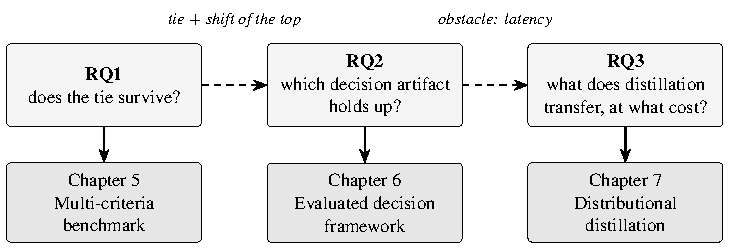
\includegraphics{images/tikz-cap1-1-en.pdf}
\caption[Research questions and chapters]{Research questions and the
chapters that answer them (the shift of the top is a consistent
lead, not a statistically confirmed separation). Source: the
author.}
\label{fig:intro-qps}
\end{figure}

\section{Summary of contributions}
\label{sec:intro-contribuicoes}

The contributions of this dissertation lie in measurement under a
uniform protocol and in openly reported evaluation --- out of sample
wherever something is learned. No new learning mechanism is claimed;
what is claimed, with dated novelty checks, is the framing and the
evidence that were missing. In order of presentation:

\begin{enumerate}
  \item \textbf{A multi-criteria benchmark of the foundation-model
    era} --- 14 models $\times$ 18 datasets (250 of the 252 cells;
    two disclosed structural exclusions), with a hold-out untouched
    by selection, frequentist and Bayesian inference and three cost
    axes under the same protocol. It yields the two facts that
    structure the dissertation: the statistical tie of the previous
    generation (8 of 10 models practically equivalent to the leader
    under the lenient criterion, 3 of 10 under the strict cutoff;
    rank variance dominated by the model$\times$dataset interaction
    together with noise)
    and the consistent lead of the 2026 generation (TabFM with the
    best rank in all three tasks and best model on 13 of 18
    datasets, zero-shot, without confirmation as a statistical
    separation by the underpowered tests, at the price of four to
    five orders of magnitude in latency). It includes the first
    neutral TabPFN~$\times$~TabFM comparison under an identical
    protocol, as far as the dated checks reach
    (Chapter~\ref{chap:benchmark}).
  \item \textbf{An independent negative result on Kolmogorov--Arnold
    networks.} In the first test of the family against the full
    GBDT (gradient-boosted decision trees)/deep
    learning/foundation-model grid in a multi-criteria benchmark
    (dated check), KAN and TabKAN finish in the bottom third on all
    three tasks, though cheap to serve: under a uniform protocol
    with tuning under paired conditions, the original papers' claims
    do not hold up (Chapter~\ref{chap:benchmark}).
  \item \textbf{A decision framework that is evaluated, not merely
    described.} Three studies evaluate the framework's components (the flowchart
    itself is their synthesis, not an evaluated policy) --- the
    learned component under leave-one-dataset-out: meta-feature
    routing does not generalize (hit rate 0.11 against 0.44 for the
    trivial baseline in the 11-model study; 0.72 against 0.78 with
    14); the fixed ``foundation model first'' policy is
    regret-optimal on the primary metric in a descriptive
    evaluation, with median regret of zero
    in the 2026 generation; and experiment E2 locates the inversion
    point (shifting 10 to 20\% of the weight from accuracy to
    latency, by median regret under the rank normalization adopted,
    is enough to flip
    the recommendation), quantitatively justifying the flowchart's
    architecture (Chapter~\ref{chap:framework}).
  \item \textbf{Distributional distillation of tabular foundation
    models.} On 20 regression datasets, under hypotheses registered
    before the experiments (Chapter~\ref{chap:destilacao}), it is
    shown that: (a) \emph{point} distillation does not work --- the
    student trained on the teacher's means beats the control on 4 of
    20 datasets with TabPFN, and the replication with TabFM as
    teacher, on the five central datasets, remains negative (a
    result reported with full prominence); (b) distilling the
    quantile curves works in part --- median retention of 12\% to
    19\% of the teacher's distributional advantage, depending on how
    the students are tuned, positive on 16 of 20 datasets (sign
    test, $p\approx0.019$ under the two-stage design correction);
    (c) the distilled student beats classical distributional
    baselines on 17 of 20 datasets (experiment E1); (d) distilling,
    compressing the context and shrinking the ensemble are measured
    on the same hold-outs, and out-of-fold labeling protects
    calibration, not accuracy; (e) these results condense into a
    decision rule whose precondition is measured in minutes. The
    dated searches of this study found no prior academic work on
    this framing (Chapter~\ref{chap:destilacao}).
  \item \textbf{Reusable infrastructure and conduct.} The protocol,
    the versioned artifacts (every number in the text traces to a
    CSV, JSON or executed notebook), the pre-registrations with
    dated addenda, the recorded novelty checks and the public
    error-correction procedure together constitute a methodological
    reproducibility contribution, described in
    Chapter~\ref{chap:metodologia} and exercised throughout the
    empirical part.
\end{enumerate}

\section{Publications}
\label{sec:intro-producao}

As of the submission of this dissertation, the research had produced
two technical reports of the graduate program, corresponding to its
individual-coursework requirements, both in English and available in
the project's public repository:

\begin{itemize}
  \item \textbf{AI-1} --- \emph{Does ``GBDT Always Win''? A
    Multi-Criteria Benchmark of 14 Tabular Models --- From a
    Statistical Tie to the 2026 Break --- and a Validated Decision
    Framework} \citep{companion2026}: technical report of the
    \emph{Trabalho Individual} (individual project) coursework
    (\texttt{latex/ai1/} in the repository), condensing the material of
    Chapters~\ref{chap:benchmark} and~\ref{chap:framework}.
  \item \textbf{AI-2} --- \emph{Distilling Tabular Foundation Models
    Beyond Classification: Distributional Regression and the
    Distill/Compress/Shrink Pareto Frontier}
    \citep{companion-ai2-2026}: technical report of the
    \emph{Atividade de Orientação Individual} (individual supervised
    research activity) (\texttt{latex/ai2/}), condensing the
    material of Chapter~\ref{chap:destilacao}; a preprint derived
    from it is being prepared for submission to arXiv.
\end{itemize}

Both reports are graded program coursework, without external peer
review as of this writing; their content corresponds, respectively,
to Chapters~\ref{chap:benchmark} and~\ref{chap:framework} and to
Chapter~\ref{chap:destilacao}, which additionally include three
contributions new to the dissertation: E2 (weighted multi-criteria
regret), entirely new relative to the reports; the complete
per-dataset results of E1 (the 17/20 paired comparison against
classical baselines; the distillation report incorporates the E1
data only through the five-system Friedman test); and the
instance-level complementarity analysis
(Section~\ref{sec:cap5-ato5}), pre-registered and executed after the
reports, which answers \emph{where} and \emph{in which cases}
foundation models beat GBDTs.

\section{How to read this dissertation}
\label{sec:intro-comoler}

The dissertation was written for three reader profiles, and not all
of them need to traverse it linearly. The \textbf{practitioner}, who
needs to choose and serve a tabular model, can go directly to
Chapters~\ref{chap:benchmark} and~\ref{chap:framework} (the evidence
and the decision flowchart) and to the decision rule that closes
Chapter~\ref{chap:destilacao} (Section~\ref{sec:destil-regra}): all
three were written to be self-contained, with the minimal
prerequisites recapped at the start of each chapter. The
\textbf{statistically minded reader} interested in the rigor of the
comparisons should start with Section~\ref{sec:fund-estatistica} of
Chapter~\ref{chap:fundamentacao} (the theory of the tests, including
the Bayesian practical-equivalence layer) and with
Chapter~\ref{chap:metodologia} (the application protocol, the policy
for missing cells and the limitations disclosed before the results).
The \textbf{replicator}, who wants to reproduce or extend the
experiments, finds in Chapter~\ref{chap:metodologia} the complete
protocol with seeds, versions and justifications, and in the
appendices the rest: the complete per-dataset tables
(Appendix~\ref{app:tabelas}), the hyperparameter search spaces
(Appendix~\ref{app:espacos-busca}) and the supplementary results and
ablations; every artifact cited has an explicit path in the
project's public repository.

\section{Structure of the dissertation}
\label{sec:intro-estrutura}

The remainder of the dissertation is organized into seven chapters
and three appendices. \textbf{Chapter~\ref{chap:fundamentacao}}
builds, from the concrete to the abstract, the technical vocabulary
of the work: tabular data and their constitutive heterogeneity,
trees and gradient boosting, the three lineages of tabular deep
learning, foundation models and the in-context-learning mechanism,
knowledge distillation, the toolkit of distributional regression
(quantiles, CRPS, calibration), the theory of statistical tests for
algorithm comparison and the decision vocabulary (algorithm
selection, regret, Pareto dominance), each at a depth proportional
to the use the later chapters make of it.
\textbf{Chapter~\ref{chap:related}} positions the work along six
axes of the literature, from tabular benchmarks to the distillation
of foundation models, closing with a synthesis table that links each
gap, characterized by dated online checks, to the chapter that
attacks it. \textbf{Chapter~\ref{chap:metodologia}} specifies the
experimental protocol shared by the whole empirical part: datasets,
models, internal selection with an untouched hold-out, metrics, the
statistical-inference protocol, cost measurement, reproducibility
infrastructure and the scientific-conduct contract, with the
design's limitations disclosed before any result.
\textbf{Chapter~\ref{chap:benchmark}} presents the benchmark in five
acts (the statistical tie of the 11-model core, the cost axes on
which the tied models differ by orders of magnitude, the conditional
reversals and the sample-size axis, the shift of the top by the 2026
generation --- a consistent lead, without confirmation as a
statistical separation --- together with the negative result on
Kolmogorov--Arnold networks, and the instance-level complementarity
between foundation models and GBDTs), answering RQ1.
\textbf{Chapter~\ref{chap:framework}} submits the decision framework
to three studies (the negative result of meta-feature routing, this
one under leave-one-dataset-out; the descriptive evaluation of the
``foundation model first'' policy; and the registered experiment on
weighted multi-criteria regret), consolidating the four-constraint
flowchart that answers RQ2. \textbf{Chapter~\ref{chap:destilacao}}
presents the distributional-distillation contribution under a
registered two-stage design: the refutation of point distillation,
the success of quantile-curve transfer, the frontier of three
serving strategies, the out-of-fold labeling ablation, experiment E1
against classical baselines and the final decision rule that answers
RQ3. \textbf{Chapter~\ref{chap:conclusao}} confronts each research
question with the accumulated evidence, consolidates the
contributions, discloses the limitations and threats to validity of
the program as a whole and points to future work. The
\textbf{appendices} gather the complete per-dataset result tables,
the hyperparameter search spaces and the supplementary results and
ablations.

%% STUB — translation pending
\chapter{Theoretical Background}
\label{chap:fundamentacao}
[Translation pending.]
\section{Pending}\label{sec:fund-estatistica}

%% STUB — translation pending
\chapter{Related Work}
\label{chap:related}
[Translation pending.]

%% STUB — translation pending
\chapter{Methodology}
\label{chap:metodologia}
[Translation pending.]
\section{Pending}\label{sec:met-metricas}

%% STUB — translation pending
\chapter{The Multi-Criteria Benchmark}
\label{chap:benchmark}
[Translation pending.]
\section{Pending}\label{sec:cap5-ato5}

%% STUB — translation pending
\chapter{The Decision Framework}
\label{chap:framework}
[Translation pending.]
\begin{equation}\label{eq:regret-normalizado}\cdot\end{equation}

%% STUB — translation pending
\chapter{Distributional Distillation}
\label{chap:destilacao}
[Translation pending.]
\section{Pending}\label{sec:destil-regra}

%% Chapter 8 --- Conclusion (English version; labels match the Portuguese deposit version).
\chapter{Conclusion}
\label{chap:conclusao}

This chapter answers the three research questions with the evidence
of Chapters~\ref{chap:benchmark} to \ref{chap:destilacao}, enumerates
the contributions --- with the negative results on the same footing
as the positive ones --- translates the results into guidance for the
practitioner, consolidates the limitations and threats to validity of
the study as a whole, and points to future work.

\section{Final remarks}
\label{sec:conc-finais}

This dissertation started from the question that organized a decade
of literature on tabular data (``do trees still win?'') and ended
answering a different one, because the evidence collected showed that
the original had expired. The three research questions stated in
Chapter~\ref{chap:introducao} receive here their direct answers, each
with the evidence of the chapter that answered it.

\textbf{RQ1} --- \emph{does the accuracy tie among the families of
tabular models survive a rigorous protocol and the arrival of the
2026 generation of foundation models?}
Chapter~\ref{chap:benchmark} answers in two beats. Within the
pre-2026 generation, yes: the top is practical equivalence gauged
under the declared criteria (8/10 equivalent under a ROPE of
$\pm0.01$ on the lenient $E[\theta]>0.5$ criterion, and 3/10 --- the
GBDTs --- at the strict 0.95 cutoff; sensitivity
$0.005/0.01/0.02 \to 2/8/10$ on the lenient criterion), with the
model$\times$dataset interaction dominating the rank variance (0.69,
against 0.20 for the family and 0.11 for the model-within-family), so
that the ``GBDT vs.\ deep learning'' axis is a weak abstraction for
these data. Across generations, no: the pre-trained paradigm pulls
away from the pack (TabFM zero-shot with average ranks 2.7/1.0/1.2 in
the three tasks --- multiclass over the two datasets where it
operates --- and best model on 13 of the 18 datasets; TabPFN as the
consistent runner-up). That lead is supported by the consistency
across datasets and the paired effect sizes --- not by the
underpowered frequentist post-hoc nor by the Bayesian instrument,
which does not separate TabFM from XGBoost and CatBoost in practical
equivalence --- and comes at the price of four to five orders of
magnitude in serving latency (43{,}262 against XGBoost's
0.33~\us/row under the standardized protocol). The instance layer (Section~\ref{sec:cap5-ato5}) further
says \emph{where} the shift lives: XGBoost and the foundation models
agree on ${\ge}93.6\%$ of instances (median), the disputed fringe is
converted in a strongly heterogeneous way across datasets, and the
easy explanations (low margin, minority class, little data) were not
confirmed under the pre-registered criteria.

\textbf{RQ2} --- \emph{which decision artifact can a benchmark with a
realistic $N$ of datasets actually support, a learned router or a
constraint-based policy --- and how does that answer change when the
decision weighs accuracy against cost?} A constraint-based policy,
not a learned router. Under leave-one-dataset-out with 18 datasets,
the meta-feature router scores below the trivial majority-class rule
(0.11 against 0.44 with 11 models; 0.72 against 0.78 with 14), even
though the conditional reversals it should exploit are real ---
recent deep learning takes the multiclass top (descriptive, $N{=}3$),
the GBDTs gain advantage under severe imbalance, TabPFN dominates the
low-data regime ($n \leq 4{,}000$; and the within-dataset subsampling
shows that the foundation models' advantage is not confined to small
datasets, Section~\ref{sec:cap5-ato5}). What the data support is a
framework of constraints verifiable before any training (latency,
architectural limits, interpretability), with the ``foundation model
first'' policy as the zero-median-regret default on the primary
metric (a descriptive evaluation, on the same 17 datasets). When the decision weighs accuracy against cost, the answer
changes early: the recommendation stops being the foundation model
between $w{=}0.9$ and $w{=}0.8$ of accuracy weight, under the rank
normalization adopted (experiment E2,
Chapter~\ref{chap:framework}) --- and that is why the flowchart's
first question is the latency budget: it is the one that changes the
answer earliest.

\textbf{RQ3} --- \emph{what does knowledge distillation transfer from
a tabular foundation model in regression, at what serving cost, and
under which conditions verifiable a priori?} It transfers part of the
shape of the predictive distribution, not the mean --- with
TabPFN-2.5 as the sole distributional teacher. The essential of what
the teacher knows about the mean, a tuned GBDT learns on its own from
the raw labels: the student trained on the teacher's means beats the
control on 4 of 20 datasets with TabPFN, and the replication with
TabFM as teacher, on the five central datasets, remains negative. The
one trained on the quantile curves retains, at the median, 19\% of
the CRPS gap with inherited hyperparameters (12\% with both arms
re-tuned) --- a median CRPS gain of 2.8\% shrinking to 1.4\% --- with
positive retention on 16 of 20 datasets (sign test,
$p\approx0.019$ under the two-stage design's sequential correction),
and beats the best of QRF and NGBoost on 17 of 20 (experiment E1).
The distributional student's serving cost is on the order of
$10^{2}$~\us{} per row in the measured frontier cases (99 and
169~\us/row; Section~\ref{sec:destil-fronteira}) --- above the point
control, and $2.5\times$ to $27\times$ below the teacher's cheapest
competitive configuration where the teacher's absolute advantage is
large. The
verifiable conditions are three, and the out-of-fold labeling that
measures them costs minutes: transform the target, test a strong
native distributional baseline, and distill only the advantage that
remains to the teacher --- with OOF labeling itself as the student's
calibration safeguard (0.5--5.1~p.p.\ of PICP80,
Chapter~\ref{chap:destilacao}).

\section{Contributions}
\label{sec:conc-contribuicoes}

The five contributions stated in
Section~\ref{sec:intro-contribuicoes} are revisited here in the same
order; under each are listed the results that compose it, with the
nature of each --- \emph{evidence} (an empirical result under a
declared protocol), \emph{framing} (a verified gap delimitation), or
\emph{rule} (an operational prescription derived from the evidence)
--- and the chapter of origin. Negative results are listed with the
same status as positive ones, per the study's conduct contract
(Chapter~\ref{chap:metodologia}).

\begin{enumerate}
  \item \textbf{The multi-criteria benchmark of the 2026 generation.}
  \begin{enumerate}
  \item \textbf{Neutral 14-model benchmark (evidence;
    Chapter~\ref{chap:benchmark}).} 14 models $\times$ 18 datasets
    (250 of the 252 cells; two structural exclusions), with a
    hold-out untouched by selection, frequentist \emph{and} Bayesian
    inference with ROPE and sensitivity analysis, and three cost
    axes under the same protocol. From it come the previous
    generation's positive tie, the shift of the top by the 2026
    generation (a consistent lead, not a statistically confirmed
    separation) and, as far as the dated checks reach, the first
    neutral TabPFN~$\times$~TabFM comparison under an identical
    protocol, framed as an inter-laboratory replication of the
    paradigm, with pinned versions and mirrored policies.
  \item \textbf{Instance-level complementarity analysis (evidence;
    Chapter~\ref{chap:benchmark}, Section~\ref{sec:cap5-ato5}).}
    Pre-registered with dated falsification criteria and exact
    reproduction of the benchmark's final models (52/52 cells
    through a sanity gate), it establishes that XGBoost and the
    foundation models agree on ${\ge}93.6\%$ of instances (median),
    that the FM's advantage is strongly heterogeneous across
    datasets (exact McNemar per pair) and, as informative negatives,
    it does not confirm the explanations of low margin, minority
    class, and advantage confined to little data (the last with a
    contrary descriptive sign in the aggregate).
  \end{enumerate}
  \item \textbf{The independent test of the Kolmogorov--Arnold
    family.}
  \begin{enumerate}
  \item \textbf{Unfavorable result under a uniform protocol
    (negative evidence; Chapter~\ref{chap:benchmark}).} In the
    family's first confrontation with the full
    GBDT/DL/foundation-model grid under a multi-criteria protocol
    --- as far as the dated checks reach --- KAN and TabKAN finish
    in the bottom third on all three tasks (ranks 11.0/12.0/9.8 and
    11.4/13.3/11.8), in line with the cost-parity critique
    \citep{kancritical2024} and against the proponents' claims ---
    and against \citet{poeta2024}'s KAN-favorable result, obtained
    without GBDT baselines and under short training, which the
    uniform protocol does not reproduce; the recorded counterpart is
    that both are cheap to serve (2.3--3.1~\us/row) --- the problem
    is performance, not cost.
  \end{enumerate}
  \item \textbf{The evaluated decision framework.}
  \begin{enumerate}
  \item \textbf{Negative result of meta-feature routing (negative
    evidence; Chapter~\ref{chap:framework}).} Under LODO with
    $N{=}18$, a learned router does not beat the majority-class
    baseline in either generation (0.11 vs.\ 0.44 with 11 models;
    0.72 vs.\ 0.78 with 14) --- corroborated by independent
    contemporary evidence \citep{herre2026}. The design consequence:
    the framework contains no winning-family predictor.
  \item \textbf{Decision framework evaluated by regret
    (evidence~$+$~rule; Chapter~\ref{chap:framework}).} The fixed
    policy ``foundation model first'' is regret-optimal on the
    primary metric (a descriptive evaluation: median regret 0.000 in
    the 2026 generation,
    preserved in the executable always-TabFM policy --- mean 0.080,
    worst case 1.000 on \texttt{telco}, the latter largely an
    artifact of the preprocessing measured in
    Chapter~\ref{chap:metodologia}), and the final framework is a
    flowchart of four constraints verifiable \emph{a priori} ---
    the form the data support.
  \item \textbf{Weighted multi-criteria regret --- E2 (evidence;
    Chapter~\ref{chap:framework}).} The registered experiment that
    locates the recommendation's inversion point: ``FM first'' is
    optimal in median only for $w \geq 0.9$ of accuracy weight;
    with $w \leq 0.6$, ``always-GBDT'' has a zero median regret. It
    is the quantitative justification of the flowchart's
    architecture --- latency is the first question because it is
    the one that changes the answer earliest.
  \end{enumerate}
  \item \textbf{The distributional distillation of tabular
    foundation models.}
  \begin{enumerate}
  \item \textbf{The framing and the central result
    (framing~$+$~evidence; Chapter~\ref{chap:destilacao}).} The
    framing --- transferring quantile curves \emph{from a tabular
    foundation-model teacher} to a GBDT student, evaluating by CRPS
    and coverage --- was verified as having no prior
    \emph{academic} work in this study's dated searches, July to
    November 2026 (complete record in
    Appendix~\ref{app:suplementares}; a public repository of
    September 2026 --- referenced in
    Section~\ref{sec:rel-destilacao} --- distills TabFM into
    XGBoost for classification and \emph{point} regression, without
    touching the distributional framing --- the non-tabular lineage
    of distributional distillation is cited as a precedent in
    Section~\ref{sec:rel-destilacao}). The evidence: median
    retention of 12\% to 19\% of the CRPS gap, depending on how the
    arms are tuned, positive on 16 of 20 datasets ($p=0.006$,
    $p\approx0.019$ under the sequential correction; Bayesian
    posterior probability of 0.96 on positive retention, with
    expected posterior mass 0.70), including a \emph{born-again}
    student (which matches its own teacher to within $10^{-4}$ of
    CRPS), serving at about a hundred microseconds per row.
  \item \textbf{Refutation of point distillation at realistic pool
    scale (negative evidence; Chapter~\ref{chap:destilacao}).} The
    distilled point student beats the control on only 4 of 20
    datasets with TabPFN; the replication with TabFM --- whose
    point advantage over the baseline is nearly $6\times$ larger on
    the measured dataset (the binarized-target
    \texttt{california\_housing}) --- remains negative on the five
    central datasets, and the pool-size sweep isolates the
    moderator (residual gain confined to $n \leq 800$,
    dataset-dependent) --- a reconciliation hypothesis with the
    contemporary point gains of \citet{jeong2026}, whose recipe
    differs from ours on axes we did not replicate (full-context
    labeling, synthetic queries, a student trained only on teacher
    predictions).
  \item \textbf{Three-strategy serving frontier (evidence;
    Chapter~\ref{chap:destilacao}).} Distilling, compressing the
    context and shrinking the ensemble measured for the first time
    on the same hold-outs: where the teacher's absolute advantage is
    large, the distilled student is, among the teacher-derived
    strategies,
    the CRPS-optimal distributional system below its cheapest
    competitive configuration ($2.5\times$ and $27\times$ the
    student's latency in the two measured cases --- E1 shows a
    native QRF also inhabits the regime); where a single-member
    teacher already reaches the student's tier, shrinking the
    ensemble suffices. Two engineering side findings: one TabPFN
    member $\approx$ eight at a seventh of the latency, and the
    last context doubling is disproportionately expensive on 16~GB
    GPUs.
  \item \textbf{Deconfounded ablation of out-of-fold labeling
    (evidence and rule; Chapter~\ref{chap:destilacao}).} In
    regression, teacher leakage does not degrade accuracy --- it
    degrades \emph{calibration} (a loss of 0.5 to 5.1~p.p.\ of
    PICP80 at identical context): a deconfounded refinement of
    Pocket~FM's classification finding \citep{pocketfm2026}.
  \item \textbf{Confrontation with classical distributional
    natives --- E1 (evidence; Chapter~\ref{chap:destilacao}).} The
    distilled student beats the best of QRF and NGBoost on 17 of 20
    datasets ($p=0.0013$, one-sided), with the three upsets
    diagnosable --- on \texttt{wine\_quality}, where the
    pre-registered gate already advised against distilling, the
    default QRF beats even the teacher. The negative complement has
    value of its own: the ``test a strong native first'' step of
    the decision rule stopped being rhetorical.
  \item \textbf{Architectural negative of TabFM as a distributional
    teacher (negative evidence; Chapter~\ref{chap:destilacao}).}
    TabFM's regression head is point-valued --- an architectural
    check of July 2026, confirmed by the official technical report
    \citep{kong2026} --- and the spread of its ensemble is
    measurably useless as a predictive distribution (CRPS 0.524
    against TabPFN's 0.069; 16.3\% coverage at a nominal 80\% ---
    measured on one dataset, the binarized-target
    \texttt{california\_housing}$^\dagger$): a
    point leader is not a distributional leader, and the
    distributional head is the decisive architectural asset for
    distillation.
  \item \textbf{Decision rule for distilling (rule;
    Chapter~\ref{chap:destilacao}).} Derived from two hypotheses
    that did not hold (point: refuted; heavy tail: not confirmed)
    and from E1: transform the target, test a strong native, and
    distill only the genuine advantage that survives --- a
    precondition measurable by a minutes-long OOF labeling. It is
    the operational form of the answer to RQ3.
  \end{enumerate}
  \item \textbf{Reusable infrastructure and conduct (transversal;
    Chapters~\ref{chap:metodologia} to~\ref{chap:destilacao}).} An
    end-to-end versioned protocol --- configurations, seeds, data
    hashes, pre-registrations with dated addenda, dated novelty
    checks and public errata --- in which every number in the text
    traces to an artifact. The contribution here is one of
    \emph{process}: the conduct contract determined concrete scope
    decisions, and its correction mechanisms were exercised in real
    cases.
\end{enumerate}

\section{Advice to the practitioner}
\label{sec:conc-conselhos}

The operational distillate of Chapters~\ref{chap:framework}
and~\ref{chap:destilacao}, in the order the questions should be
asked --- each item traces to the result that supports it.

\begin{itemize}
  \item \textbf{Start from the constraints, not from performance.}
    Four questions verifiable before any training: latency budget,
    architectural limits, interpretability requirement, and only
    then the default (flowchart of
    Section~\ref{sec:arcabouco-resultante}). Do not try to learn a
    meta-feature router with a few dozen datasets: under LODO, it
    does not beat the trivial rule
    (Section~\ref{sec:resultado-negativo}).
  \item \textbf{If microsecond latency matters, GBDT.} With 40\% or
    more of the utility weight on latency, ``always-GBDT'' has a
    zero median regret; the ``FM first'' recommendation already
    flips with 10--20\% of the weight on latency (by the median;
    E2, Section~\ref{sec:regret-ponderado}).
  \item \textbf{If no constraint is active, foundation model
    first.} Median regret 0.000 in the 2026 generation
    (Section~\ref{sec:resultado-positivo}) --- with TabPFN as the
    mature option and TabFM as the frontier, at the versions and
    with the maturity caveats declared in
    Chapter~\ref{chap:benchmark}.
  \item \textbf{Check the architectural limits early.} More than 10
    classes excludes TabFM; 100 classes exclude both foundation
    models (the \texttt{helena} case); context overflow is an
    objective restriction --- these are structural exclusions, not
    details (Section~\ref{sec:arcabouco-resultante}).
  \item \textbf{In regression with uncertainty: transform before
    distilling.} On price-scale targets, a one-line logarithmic
    transformation is free and changes the error regime of every
    system --- it does not eliminate the teacher's relative
    advantage, but it is the first test to run, and it costs
    minutes (Section~\ref{sec:destil-regra}).
  \item \textbf{Test the QRF before distilling.} A default
    distributional native costs seconds of training, serves at
    microseconds and, on a predictable minority of datasets,
    settles the problem before any teacher needs to be loaded ---
    on \texttt{wine\_quality}, it beat even the teacher (E1,
    Section~\ref{sec:destil-e1}); a quantile MLP covers the small,
    numeric datasets (Section~\ref{sec:destil-regra}).
  \item \textbf{Distill when the advantage survives the
    transformations and a strong native --- and measure it first.}
    A single OOF labeling, at a cost of minutes, directly measures
    the teacher's genuine advantage; distill only if it persists
    (Section~\ref{sec:destil-regra}). Do not distill the mean: at
    realistic pools, there is nothing to transfer on the point axis
    (Section~\ref{sec:destil-ponto}).
  \item \textbf{Always label out-of-fold.} The cost is modest, and
    the safeguard protects what accuracy metrics do not see: the
    student's interval coverage (0.5--5.1~p.p.\ of PICP80;
    Section~\ref{sec:destil-oof}).
  \item \textbf{Before paying for the full teacher, shrink the
    ensemble.} A single TabPFN member approximated the eight at a
    seventh of the latency --- sometimes at no accuracy cost ---
    and, when a single teacher member already reaches the student's
    latency tier, that lever closes the case without any
    distillation (Section~\ref{sec:destil-fronteira}).
  \item \textbf{On 16~GB GPUs, distrust the last context
    doubling.} The final doubling, from 25{,}000 to 50{,}000 rows,
    cost $3.3\times$ the latency for a marginal accuracy gain
    (Section~\ref{sec:destil-fronteira}); reserve the full-context
    teacher for batch processing.
\end{itemize}

The list above orders the questions; it remains to name the
scenarios. Table~\ref{tab:conc-perfis} consolidates the same results
as \emph{usage profiles}: for each condition --- six of the ten
verifiable before any training, the rest after one cheap, declared
measurement --- the recommendation the data support, the measured
evidence
that supports it and --- the column the usual benchmarks omit ---
what one accepts to lose in exchange. The final column is the point:
in several profiles, the recommendation is deliberately a model
\emph{worse on the primary metric}, and the trade is defensible
because it was measured. Two results support this accounting: in the
core's pack, giving up the top typically costs less than one
percentage point of AUC (Section~\ref{sec:cap5-ato1}), while the
differences in latency, minority-class recall, and tail cost are of
whole factors to orders of magnitude (columns 3 and 4 of the table).
When the metric on which the models differ is the one the
application pays, it is the one that decides --- and the table says
which it is, case by case.

\begin{table}[htbp]
\centering
\caption[Usage profiles: condition, recommendation, evidence, and
trade]{Usage profiles: verifiable condition, recommendation,
evidence, and accepted cost in exchange. Source:
Chapters~\ref{chap:benchmark}--\ref{chap:destilacao}, sections
indicated.}
\label{tab:conc-perfis}
\scriptsize
\setlength{\tabcolsep}{5pt}
\renewcommand{\arraystretch}{1.15}
\begin{tabular}{p{0.21\linewidth}p{0.17\linewidth}p{0.33\linewidth}p{0.19\linewidth}}
\toprule
\textbf{Profile (condition)} & \textbf{Recommendation} &
\textbf{Evidence} & \textbf{Accepted in exchange} \\
\midrule
No active constraint; latency-tolerant &
Foundation model first (TabPFN mature; TabFM frontier) &
Median regret 0.000 with 14 models in
Chapter~\ref{chap:framework}'s evaluation (the family's ceiling,
measured on the same 18 datasets; the executable always-TabFM
preserves the median, with mean 0.080 and worst case 1.0;
always-TabPFN: median 0.242); absolute best on 13 of 18
(Sections~\ref{sec:resultado-positivo}, \ref{sec:cap5-ato4}) &
Serving cost (from ${\sim}3{,}900\times$ the slowest GBDT ---
TabPFN over LightGBM, Table~\ref{tab:app-custos} --- to
$131{,}097\times$ XGBoost); TabPFN-2.5's non-commercial license \\
\addlinespace
Little data ($n \lesssim 4{,}000$) &
TabPFN &
Average rank 1.0 in the regime, against XGBoost's 2.8, on the 5
swept datasets (Section~\ref{sec:cap5-ato3}) &
Inference latency; large-$n$ leadership depends on the dataset \\
\addlinespace
Rare class with expensive false negatives &
FM at a fixed threshold --- \emph{or} re-optimize the GBDT's
threshold; measure recall at equalized precision before switching &
\texttt{amazon\_employee}: accuracies 0.943--0.949
indistinguishable; minority recall 0.032 $\to$ 0.298 at threshold
0.5 (Section~\ref{sec:cap5-ato5}). Counterweights: the
rare-class-gain hypothesis was not confirmed; the dataset's best AUC
belongs to a GBDT (CatBoost 0.887, Table~\ref{tab:app-binaria}) ---
a fixed-threshold advantage, on one dataset &
Precision (0.706 $\to$ 0.621) and latency; the advantage is
frequent, not law (\texttt{give\_me\_some\_credit}: recalls that
differ by less than 0.02 from one another) \\
\addlinespace
Regression with tail decisions and a \us{} budget &
Distilled student (conformal coverage correction: piloted on 5
datasets) &
Positive retention on 16/20 ($p{=}0.006$ single-stage; $0.019$
sequential), held
re-tuned; at $\tau{=}0.90$, 18/20 ($p{=}0.0002$), ${\sim}8\%$ gain
in the tails; the distilled$+$conformal combination not measured
jointly on the 20 (Sections~\ref{sec:destil-dist},
\ref{sec:destil-e3}) &
Nothing on the point axis (4 of 20); latency above the control, on
the order of $10^2$~\us{} per row; the OOF pipeline; the teacher's
non-commercial license reaches the distilled student \\
\addlinespace
The application's metric inverts the winner &
Decide by the metric the application pays; report both layers &
\texttt{telco}: TabFM loses accuracy (0.771 vs.\ 0.801) and the
McNemar fringe ($-29.8$/thousand), but wins recall (0.663 vs.\
0.570) and balanced accuracy (0.737 vs.\ 0.727)
(Section~\ref{sec:cap5-ato5}) &
The primary metric's ``winner''; an unoptimized threshold; and
\texttt{TotalCharges} (Ch.~4) reaches this dataset: with the column
numeric, TabFM jumps from last to best AUC among the 14 re-evaluated \\
\addlinespace
Advantage heterogeneous per dataset (instance-level disagreement
fringe, Section~\ref{sec:cap5-ato5}) &
Choose per dataset/task, never per instance; no learned router &
Agreement $\geq$0.936; TabFM converts the fringe on \texttt{jannis}
($+59.6$/thousand) and loses it on \texttt{telco}; the LODO router
below the trivial rule (Sections~\ref{sec:cap5-ato5},
\ref{sec:resultado-negativo}) &
The promise of ``a universal winner''; the advantage does not
shrink with size \\
\addlinespace
Microseconds-per-row latency required &
Native GBDT; distillation recovers part of the distributional
advantage &
0.33~\us/row (XGBoost) vs.\ 43{,}262 (TabFM), $131{,}097\times$;
the FM recommendation flips with 10--20\% of latency weight (by
median regret; E2)
(Sections~\ref{sec:cap5-ato2}, \ref{sec:regret-ponderado}) &
The top rank --- a loss $<$1~p.p.\ of AUC in the core's pack (ROPE
vs.\ TabPFN: 8/10 lenient, 3/10 strict); vs.\ TabFM the equivalence
is uncertain ($P$ 0.33; $E[\theta]$ 0.40) \\
\addlinespace
Intrinsic interpretability required (regulation) &
GBDT &
The only family strong in latency \emph{and} interpretability in
the multi-criteria matrix --- a qualitative per-family attribution,
declared, not measured; gate 3 of the flowchart
(Section~\ref{sec:arcabouco-resultante}) &
The top rank, under the same ROPE accounting; no distillation (the
student inherits labels from an opaque teacher) \\
\addlinespace
Architectural limit ($>$10 classes; context overflow) &
GBDT or recent DL depending on the task &
\texttt{helena} (100 classes) excludes both FMs; descriptive
multiclass top: STab/TabM 3.67 vs.\ XGBoost 6.0, $N{=}3$
(Sections~\ref{sec:cap5-ato3}, \ref{sec:arcabouco-resultante}) &
Nothing: the exclusion is structural, not a preference \\
\addlinespace
Small teacher advantage; price-scale target; strong native
available &
Do \emph{not} distill: QRF first, $\log(1{+}y)$, ensemble
shrinking &
E1: the QRF beats the distilled student on 3 of 20 (on
\texttt{wine\_quality}, even the teacher); \texttt{kin8nm}: 1
member at the student's latency; the log changes the error regime
for free, without eliminating the teacher's relative advantage
(Sections~\ref{sec:destil-e1}, \ref{sec:destil-fronteira},
\ref{sec:destil-regra}) &
The whole distillation pipeline --- and that is a gain, not a loss \\
\bottomrule
\end{tabular}
\end{table}

Three readings close the table. First, in the profiles where the
recommendation goes against the primary metric (latency,
interpretability, rare class), the trade is accounted for in the two
final columns: the loss on the primary is bounded by measurement (by
the ROPE in the pack, by the declared threshold in the operational
metrics), while the gain on the application's metric is of whole
factors to orders of magnitude. Second, the negative profiles are as
informative as the positive ones: the table says when \emph{not} to
use the foundation model (microseconds, 100 classes, regulation) and
when \emph{not} to distill (\texttt{kin8nm},
\texttt{wine\_\allowbreak quality}), with the cases measured in the
benchmark itself. Third, no row is a ranking: six are conditions
known before any training, in the form Chapter~\ref{chap:framework}
evaluated; the other four (rare class, metric inversion,
instance-level fringe, teacher advantage) call for a cheap, declared
measurement --- a second metric on the hold-out, an out-of-fold
labeling --- before deciding.

\section{Limitations and threats to validity}
\label{sec:conc-limitacoes}

Each chapter declared its local limitations; this section
consolidates those of the study as a whole, organized by the three
canonical validity types (Section~\ref{sec:met-limitacoes}). Two
transversal limitations enter the taxonomy with their own
prominence: multiplicity and the pure distilled student's
undercoverage, below, under internal validity; the teachers'
licenses, under external validity.

\subsection{Internal validity}

\textbf{Benchmark-aware priors --- the unaddressable residual
risk.} TabFM declares exclusively synthetic pre-training; the
default TabPFN v2.5 classifier checkpoint, however, is fine-tuned
on 43 real datasets that include this benchmark's \texttt{higgs}
--- and, by a name match not verified row by row, probably
\texttt{cardiovascular\_disease} --- (with the sensitivity measured
on the twelve classification datasets: AUC differences between
$-0.0051$ and $+0.0002$, and on \texttt{higgs} the synthetic-only
checkpoint is even slightly better, 0.8113 against 0.8111;
Section~\ref{sec:met-limitacoes}); the default regressor is purely
synthetic, preserving the distributional part. There remains,
beyond that, the weaker risk of priors and inference policies
iteratively tuned, across versions, to performance on public
benchmarks: a mild form of community overfitting from which no
public benchmark escapes. The treatment was to declare the risk,
state conclusions at the regime level (consistency across datasets,
not individual cells), and keep the cost axis, immune to
contamination, in every practical conclusion
(Section~\ref{sec:met-limitacoes}).

\textbf{Declared asymmetries in the complementary experiments.} In
E1, NGBoost and the QRF run in documented default configuration,
without specific tuning, and the QRF receives median imputation
(fitted on the pool, applied to the test) on the three datasets with
missing values; the licensed interpretation is ``strong default'',
not ``classical tuned to the limit''
(Section~\ref{sec:destil-e1}). In the distillation students,
capacity is inherited from the benchmark's tuning, with no
re-tuning per distillation target --- a deliberate control, with
the declared caveat that between the arms both the label \emph{and}
the loss change; the asymmetry's cost was measured by the
re-tuning, registered in a dated addendum before execution, on the
20 datasets: the aggregate verdict survives the re-tuned control
(16 of 20, median 0.124 against the inherited 0.192, a declared
drop), leaving per-dataset retention dependent on the tuning budget
(Section~\ref{sec:destil-retune}). Related design-level caveats are
consolidated where they are declared: the non-nested selection
design --- a property of the benchmark (RQ1) that RQ3 inherits
through the students' hyperparameters --- with its optimism
quarantined to internal roles, in
Section~\ref{sec:met-protocolo}; the single distributional teacher
(TabPFN-2.5) and the regression-only scope, in
Chapter~\ref{chap:destilacao}'s limitations and synthesis.

\textbf{Dataset-identity errors.} Two labeling errors inherited
from the project's creation (\texttt{diamonds}/\texttt{kin8nm};
``superconduct''/\texttt{online\_news}) were discovered during the
study and corrected with re-derivation of all affected numbers;
every number in this dissertation postdates the corrections
(Section~\ref{sec:met-datasets}; record in
Appendix~\ref{app:suplementares}). The residual threat is the one
corrections do not remove: the possibility of analogous errors not
yet discovered; the mitigation is structural (data hashes,
versioned configurations, numbers traceable to artifacts).

\textbf{Multiplicity across experiments.} No correction is applied
\emph{across} experiments; under Holm correction on the
confirmatory family, the primary conclusions survive and the
supplementary instruments do not --- and RQ3's headline carries the
sequential correction of its two-stage design ($p\approx0.019$;
Section~\ref{sec:destil-desenho}).

\textbf{Undercoverage of the pure distilled student.} The
pre-registered coverage clause (PICP80 within $\pm5$~p.p.\ of
nominal) is met on only 10 of the 20 datasets --- the answer to RQ3
is qualified by this: the calibration gain is comparative, and the
closing of coverage comes from the conformal step, piloted on 5
datasets (Section~\ref{sec:destil-dist}).

\subsection{External validity}

\textbf{Small $N$ per task and the arithmetic floors.} With 10/3/5
datasets per task, the tests' power is low by construction: in
regression, the smallest two-sided Wilcoxon p-value is 0.0625
(significance at 5\% is mathematically impossible, before any
correction) and multiclass ($N{=}3$) is treated as descriptive
throughout the text. The declared mitigations (equivalences
supported by the Bayesian layer, no conclusion resting on
significance where there is no power) limit the damage but do not
eliminate it: the per-task conclusions have the precision $N$
allows, no more (Section~\ref{sec:met-limitacoes}).

\textbf{The double exclusion of \texttt{helena}.} The two
foundation models' multiclass ranks are averages over only 2
datasets, a fact repeated in every affected table. The alternative
(removing the dataset) would hide exactly the kind of architectural
restriction a practical decision study should expose; the price is
that the 2026 generation's multiclass lead rests on the smallest
sample base of the whole benchmark.

\textbf{TabFM at a pinned version, with an unreviewed technical
report.} All results refer to version v1.0.1 (July 2026, pinned
commit); the official technical report \citep{kong2026} appeared in
late September 2026 and, as of this writing, has not undergone peer
review \citep{tabfm2026}. The conclusions about the model are about
\emph{that} version; and version sensitivity is itself future work
(Section~\ref{sec:conc-futuros}).

\textbf{Delimited regime.} Eighteen OpenML datasets (plus the
fifteen of the CTR23 extension in the distillation), a
100{,}000-sample cap and a single 16~GB GPU delimit the regime
studied to small-and-medium tabular data on commonly sized
hardware. Four eligible CTR23 datasets stayed outside the
distillation population; the sensitivity with them, measured on
five data splits, keeps the verdict (17/24, $p=0.032$; conservative
cut 16/22, $p=0.026$; Chapter~\ref{chap:destilacao}). The orders of
magnitude between families tend to transfer; the absolute values do
not.

\textbf{The field moves in cycles of months.} TabPFN-2.5 in
November 2025, Pocket~FM in May 2026, TabFM in June, the partial
collision of \citet{jeong2026} in October; the difference between
the @11 and @14 columns of the LODO evaluation is the internal
demonstration of how fast conclusions date. For this reason every
novelty claim and every gap characterization carries a verification
date, from this study's dated searches, July to November 2026
(complete record in Appendix~\ref{app:suplementares}), and must be
read as ``open as far as we checked, at the declared dates'', never
as timeless certainty (Chapter~\ref{chap:related}).

\textbf{The binarized target in the regression core.} The core's
\texttt{california\_\allowbreak housing} is the binarized-target
variant of the \emph{tabular-benchmark} --- degenerate for
distributional claims. Every headline distillation result carries a
sensitivity analysis with the dataset excluded: the sign test, E3,
the five-system Friedman, and the ablations survive; the one-sided
Wilcoxon of the retention moves from $0.045$ to $0.067$ and stops
rejecting at 5\%, a degradation declared with the same prominence
as the result (Chapter~\ref{chap:destilacao}).

\textbf{Teacher licenses.} The weights of TabPFN-2.5 and TabFM are
non-commercial, and TabPFN's license further forbids distilling
from its outputs a ``competitive'' model; this study's distilled
student operates in a research regime, and commercial deployment
would require its own licensing
(Section~\ref{sec:destil-limitacoes};
Appendix~\ref{app:suplementares}).

\subsection{Construct validity}

\textbf{The \texttt{adult} latency proxy.} Latency enters the
analyses (including E2's weighted score) through the standardized
measurement in a single regime (amortized batch, each model on its
natural device), with \texttt{adult} as the reference. The bias
direction was declared in the registration and its magnitude was
later measured at the benchmark's size extremes: the rankings among
the 14 models are stable across datasets (Spearman 0.78--0.95) and
E2's crossover is identical under the three proxies
(Sections~\ref{sec:met-limitacoes}
and~\ref{sec:regret-ponderado}). What remains unmeasured is
hardware sensitivity: all numbers come from a single declared
machine.

\textbf{The grid CRPS estimator.} The 19-quantile grid
overestimates the exact CRPS by a nearly constant ${\sim}$4--5\%,
validated against the Gaussian closed form: internal comparisons
and retention ratios are preserved, but this dissertation's
absolute CRPS values should not be compared to other works'
(Section~\ref{sec:destil-metricas}).

\textbf{Metrics compress utilities.} The threshold-free primary
metric and E2's score (two criteria, linear weights) are
deliberately simple constructs of utility functions that, in
practice, include training cost, robustness, interpretability, and
regulatory constraints with non-linear weights. The framework keeps
the axes separate instead of aggregating them prematurely, but any
scalar recommendation inherits that compression
(Sections~\ref{sec:met-limitacoes}
and~\ref{sec:limitacoes-framework}).

\section{Future work}
\label{sec:conc-futuros}

Only directions with direct grounding in the chapters' evidence are
listed (extensions this study leaves ready, not speculations).

\begin{itemize}
  \item \textbf{Newer teachers: version sensitivity of the
    distillation.} The study pinned TabPFN v2.5 for comparability
    with the benchmark; TabPFN-3 and 3.5
    \citep{tabpfn3-2026,tabpfn35tr2026} already exist, and the
    partial collision of \citet{jeong2026} (point gains with newer
    teachers, under a different protocol) suggests the
    teacher--student frontier is version-sensitive. Repeating the
    distributional protocol with the next generation's teachers
    would directly measure whether the 12--19\% retention grows
    with the teacher's strength --- and whether the point negative
    resists.
  \item \textbf{Conformal calibration as complement and
    competitor.} The post-hoc conformal route on the teacher
    itself \citep{park2026} delivers coverage guarantees without a
    fast student --- at the price of the foundation model's
    latency. Incorporating it into the frontier (and applying it on
    the distilled student beyond the five-dataset pilot of
    Appendix~\ref{sec:app-pilot-conformal}) would test the
    calibration advantage observed in
    Section~\ref{sec:destil-oof} against a method with a formal
    guarantee.
  \item \textbf{Quantization as the frontier's fourth arm.}
    Attention quantization \citep{kubler2026} is the emerging
    serving lever we did not measure; the three-strategy frontier
    of Section~\ref{sec:destil-fronteira} is built to receive it
    as a fourth arm on the same hold-outs.
  \item \textbf{Multi-criteria regret with elicited preferences.}
    E2 swept linear weights over two criteria, and the latency
    proxy's robustness to the measurement dataset has been
    verified (Section~\ref{sec:regret-ponderado}); the natural
    extension is to incorporate training cost, robustness, and
    interpretability into the score and elicit utility functions
    from real practitioners --- testing whether the inversion
    point (10--20\% of latency weight, by median regret) moves with
    additional criteria.
  \item \textbf{KANs under dedicated tuning.} The negative result
    of Chapter~\ref{chap:benchmark} uses the grid's uniform
    protocol --- the fair reading for the benchmark's question,
    but not the last word on the family: a dedicated study, with
    its own search budget, the original optimizer, and basis
    variants, would definitively separate method from recipe ---
    and would say whether the bottom third is a ceiling or a
    protocol artifact.
  \item \textbf{A living update of the benchmark.} The resumable
    infrastructure, with pinned versions and seeds, is ready for
    periodic re-execution as the 2027 generation arrives;
    integration with a community-maintained living benchmark, in
    the style of TabArena \citep{tabarena2025}, is the path for
    this study's protocol depth to survive its dating --- the main
    external threat declared above.
\end{itemize}

\vspace{1em}

In synthesis, the dissertation delivers three pieces: a dated
benchmark of the 2026 generation, with the cost axes measured under
the same conditions as accuracy; a constraint framework evaluated
out of sample in its learned component, with the cost-driven
inversion point located; and a rule, tested also in its failures,
for deciding when to distill a foundation model's predictive
distribution into a student that serves at about a hundred
microseconds per row. All three depend on the declared model
versions, datasets, and hardware, and must be re-evaluated when
they change; the public protocol, with versioned seeds, artifacts,
and errata, exists so that this re-evaluation, and any correction
it brings, costs little to whoever comes next.


\cleardoublepage
\markboth{REFERENCES}{REFERENCES}
\bibliographystyle{abnt}
\bibliography{references}

\theappendix
%% STUB
\chapter{Complete result tables}
\label{app:tabelas}
[Translation pending.]

%% STUB
\chapter{Hyperparameter search spaces}
\label{app:espacos-busca}
[Translation pending.]
\section{Pending}\label{app:hp-escolhidos}

%% STUB
\chapter{Supplementary results}
\label{app:suplementares}
[Translation pending.]
\section{Pending}\label{sec:app-abl-sort}
\section{Pending}\label{sec:app-pilot-conformal}


\end{document}
